\section*{\begin{center}{\Huge Appendix}\end{center}}
\addcontentsline{toc}{chapter}{Appendix}
$\\[0.5cm]$

\noindent Write your appendix here...

\todo[inline]{Include confusion matrices for the remaining data sets}
 
\section{Additional Results}

\subsection{Measuring error rate}

\begin{table}[H]
	\centering
	\begin{tabular}{|l|l|l|l|}
		{\bf Experiment Name}            & {\bf Mean error} & {\bf Std. dev.} & {\bf $\lambda$} \\
		\hline
		Centralized logistic regression  & $0.104$          & $0.0059$        & $2^{-8}$        \\
		Disjoint logistic regression     & $0.159$          & $0.0026$        & $2^{-5}$        \\
		Aggregated model, $\epsilon=1.0$ & $0.163$          & $0.0103$        & $2^{-3}$        \\
		Ensemble model, $\epsilon=1.0$   & $0.150$          & $0.0045$        & $2^{-5}$        \\
		Aggregated model, $\epsilon=0.1$ & $0.182$          & $0.0256$        & $2^{-1}$        \\
		Ensemble model, $\epsilon=0.1$   & $0.157$          & $0.0117$        & $2^{-2}$       
	\end{tabular}
	\caption{Measuring accuracy: Spambase}
	\label{tab:results_measuring_accuracy_spam}
\end{table}

\subsection{Changes in number of participants}


\begin{figure}[H]
	\centering
	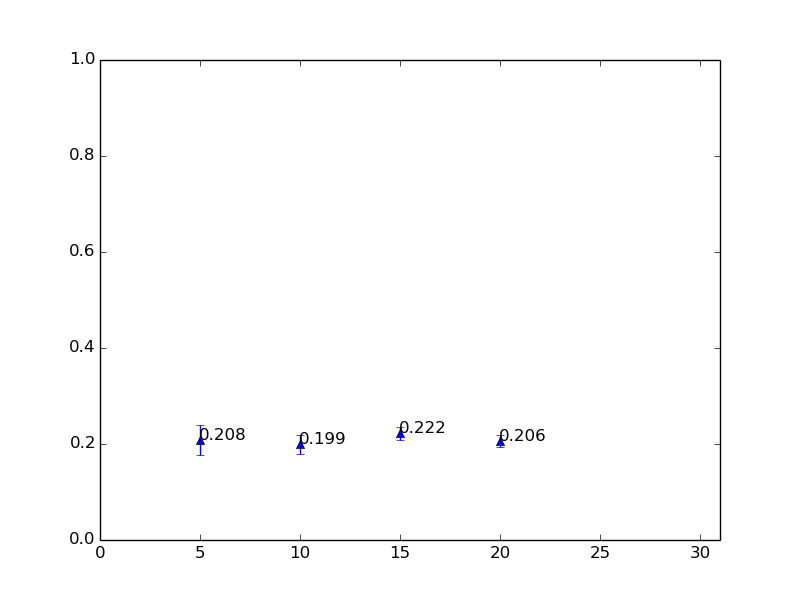
\includegraphics[width=\textwidth]{fig/spambase/eps1.0,bud1.0,peers5-30,groups5,reg2e-2-puball-peercounts-data150-spam-testmean}
	\caption{Effect of peer numbers. Spambase.}
	\label{fig:peer_range_constant_group_spam}
\end{figure}